\documentclass[tikz,border=10pt]{standalone}
\usepackage{amsmath}
\usetikzlibrary{arrows.meta, positioning, calc, decorations.pathreplacing}
\definecolor{c1}{HTML}{000000}
\definecolor{c2}{HTML}{233D4D}
\definecolor{c3}{HTML}{FE7F2D}
\definecolor{c4}{HTML}{EAECF0}
\definecolor{axiscolor}{HTML}{333333}
\definecolor{labelcolor}{HTML}{5F6B75}
\begin{document}
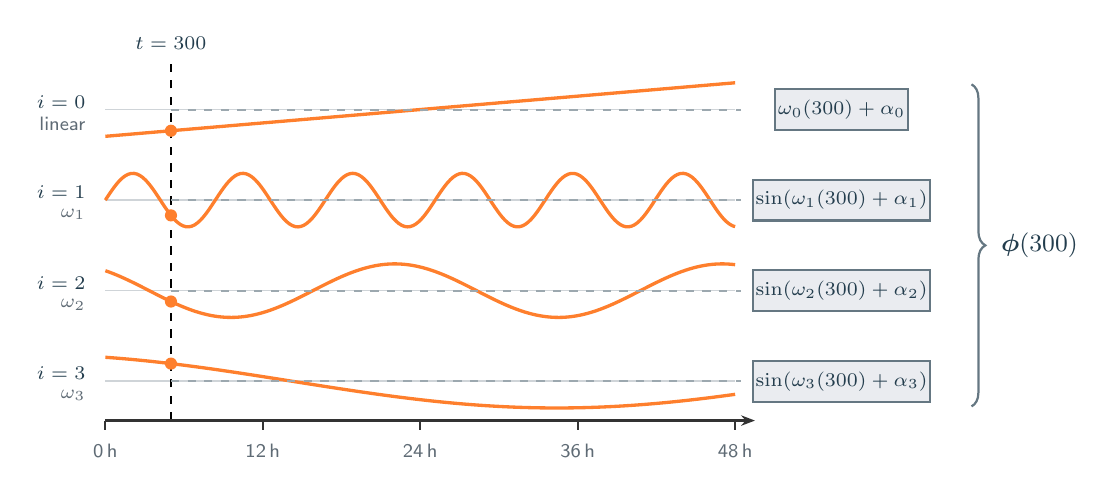
\begin{tikzpicture}[
    every node/.style={font=\sffamily},
    lab/.style={font=\sffamily\scriptsize, text=labelcolor},
    tag/.style={font=\sffamily\scriptsize, text=c2},
    guide/.style={c2!45, line width=0.7pt, dashed},
    cell/.style={rectangle, draw=c2!70, fill=c4, line width=0.8pt,
                 minimum width=1.35cm, minimum height=0.52cm,
                 font=\sffamily\scriptsize, text=c2, inner sep=1pt},
]
\def\X#1{1.55 + #1*0.002778}

% ---------------------------------------------------------------- the terms
% i = 0, the linear term
\node[tag, anchor=east] at (1.42, 5.70) {$i = 0$};
\node[lab, anchor=east] at (1.42, 5.42) {linear};
\draw[c2!22, line width=0.6pt] (1.55, 5.60) -- (9.55, 5.60);
\draw[c3, line width=1.2pt] ({\X{0}}, {5.60-0.34}) -- ({\X{2880}}, {5.60+0.34});

% three learned waves
\foreach \y/\i/\w/\a in {4.45/1/0.0125/0, 3.30/2/0.0042/40, 2.15/3/0.0013/90}{
    \node[tag, anchor=east] at (1.42, {\y+0.10}) {$i = \i$};
    \node[lab, anchor=east] at (1.42, {\y-0.18}) {$\omega_\i$};
    \draw[c2!22, line width=0.6pt] (1.55, \y) -- (9.55, \y);
    \draw[c3, line width=1.2pt]
        plot[domain=0:2880, samples=220, smooth]
        ({\X{\x}}, {\y + 0.34*sin((\x*\w + \a) r)});
}

% ---------------------------------------------------------------- one time
\draw[c1, line width=0.8pt, dashed] ({\X{300}}, 1.65) -- ({\X{300}}, 6.20);
\node[tag, anchor=south] at ({\X{300}}, 6.24) {$t = 300$};
\fill[c3] ({\X{300}}, {5.60-0.34+0.0708}) circle (2.2pt);
\fill[c3] ({\X{300}}, {4.45 + 0.34*sin((300*0.0125) r)}) circle (2.2pt);
\fill[c3] ({\X{300}}, {3.30 + 0.34*sin((300*0.0042 + 40) r)}) circle (2.2pt);
\fill[c3] ({\X{300}}, {2.15 + 0.34*sin((300*0.0013 + 90) r)}) circle (2.2pt);

% ---------------------------------------------------------------- the vector
\node[cell] (v0) at (10.90, 5.60) {$\omega_0 (300) + \alpha_0$};
\node[cell] (v1) at (10.90, 4.45) {$\sin(\omega_1 (300) + \alpha_1)$};
\node[cell] (v2) at (10.90, 3.30) {$\sin(\omega_2 (300) + \alpha_2)$};
\node[cell] (v3) at (10.90, 2.15) {$\sin(\omega_3 (300) + \alpha_3)$};
\foreach \y in {5.60, 4.45, 3.30, 2.15}{
    \draw[guide] ({\X{300}}, \y) -- (9.62, \y);
}
\draw[decorate, decoration={brace, amplitude=5pt}, c2!70, line width=0.8pt]
    (12.55, 5.92) -- (12.55, 1.83)
    node[midway, right=7pt, font=\sffamily\small, text=c2] {$\boldsymbol{\phi}(300)$};

% ---------------------------------------------------------------- axis
\draw[axiscolor, line width=0.8pt, -{Stealth[length=5pt]}] (1.55, 1.65) -- (9.80, 1.65);
\foreach \h in {0, 12, 24, 36, 48}{
    \pgfmathsetmacro\m{\h*60}
    \draw[axiscolor, line width=0.7pt] ({\X{\m}}, 1.65) -- ({\X{\m}}, 1.53);
    \node[lab, anchor=north] at ({\X{\m}}, 1.47) {\h\,h};
}
\end{tikzpicture}
\end{document}
